\begin{EXTRA}[./golden-ratio.png]{فیبوناچی و نسبت طلایی }
    \p
    به شکل زیر دقت کنید، اگر گیاه از هر گره ۲ ماه زمان لازم داشته باشد تا دوشاخه شود، تعداد ساقه‌های این گیاه در آخر هر ماه از دنباله فیبوناچی پیروی می‌کند(چرا؟).
    
    \centerimage{0.4}{./sneezewort.jpeg}
    \p
    وجود الگوی رشد بالا در طبیعت باعث شده عدد فیبوناچی به کرات مشاهده شوند.
    در اکثر گل‌ها تعداد گلبرگ‌ها ۳ ، ۵ ، ۸ ، ۱۳ و .. است.
    \centerimage{0.4}{./flower3.jpg}
    \p
    با قرار دادن مربع‌هایی به ضلع اعداد فیبوناچی در کنار هم و اتصال رئوس این مربع‌ها به کمک کمان،\FOCUSEDON{مارپیچ فیبوناچی} تشکیل می‌شود.
    \centerimage{0.4}{./Fibonacci.jpeg}
    \p
    مجددا با توجه به الگوی رشد فیبوناچی، مارپیچ فیبوناچی به کرات مشاهده می‌شود.
    مارپیچ گوش انسان،لاک حلزون و ساختار مارپیچ کهکشان‌ها نمونه‌هایی از مارپیچ فیبوناچی هستند.
    \centerimage{0.2}{./earFibonacci.jpeg}
    \centerimage{0.3}{./mollusc.jpeg}
    \centerimage{0.4}{./galaxy.jpeg}
    % \begin{figure}
    %     \centering
    %     \begin{subfigure}[b]
    %         {0.3\textwidth}
    %         \centering
    %         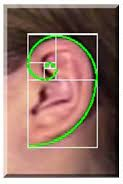
\includegraphics[width=\textwidth]{./earFibonacci.jpeg}
    %     \end{subfigure}
    %     \hfill 
    %     \begin{subfigure}[b]
    %         {0.3\textwidth}
    %         \centering
    %         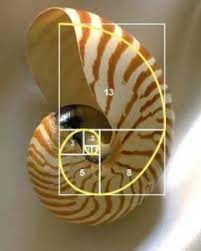
\includegraphics[width=\textwidth]{./mollusc.jpeg}
    %     \end{subfigure}
    %     \hfill
    %     \begin{subfigure}[b]
    %         {0.3\textwidth}
    %         \centering
    %         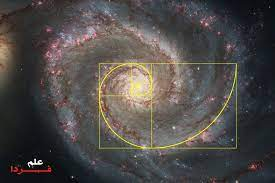
\includegraphics[width=\textwidth]{./galaxy.jpeg}
    %     \end{subfigure}
    % \end{figure}
    \p
    شاید با نسبت طلایی آشنا باشید. به مقدار $\frac{1+\sqrt{5}}{2}$ نسبت طلایی گفته می‌شود.
    شایان ذکر است که نسبت دو جمله متوالی دنباله فیبوناچی به سمت نسبت طلایی همگرا می‌شود.
    این همگرایی را می‌توان به شکل زیر اثبات کرد.
    اثبات:

    \p
    واضح است که نسبت طلایی پاسخ معادله
    $x^2-x-1=0$
    است که برابر عبارات
    $1+\frac{1}{1+\frac{1}{1+...}}$
    و
    $\sqrt{1+\sqrt{1+\sqrt{...}}}$
    نیز می‌باشد.
    آیا می‌توانید این برابری را اثبات کنید؟
    \p
    با توجه به وفور الگوی رشد فیبوناچی در طبیعت و رابطه این دنباله با نسبت طلایی، این مقدار نیز زیاد در طبیعت دیده می‌شود.
    مثلا:
    لئوناردو داوینچی با اندازه‌گیری نسبت دقیق استخوان‌های انسان ثابت کرد این نسبت ضریبی از عدد طلایی است.
    اگر قد خود را بر فاصله عمودی ناف تا نوک انگشتان خود تقسیم کنید، تقریبا نسبت طلایی را بدست می‌آورید.
    با تقسیم طول بازوی خود از نوک انگشت بزرگ تا بالای شانه، بر فاصله نوک انگشت بزرگ تا آرنج خود نیز به این نسبت می‌رسید.
    جالب است اگر به چرایی ظاهر شدن دنباله فیبوناچی و نسبت طلایی در طبیعت تحقیق و تفکر کنید.
    \p
    علاوه بر طبیعت، از زمان باستان بسیاری از هنرمندان و معماران نیز از رابطه‌های ریاضی و هندسی در آثار خود به دلیل استحکام و زیبایی استفاده می‌کردند.
    معبد معروف پارتنون بهترین مثال از کاربرد نسبت طلایی است. نسبت عرض به طول پنجره‌های مستطیل شکل معبد همگی برابر نسبت طلایی است.

\end{EXTRA}